\chapter{Spherical SfM}
\lhead{\chaptername~\thechapter. \emph{Spherical SfM}}
In this chapter, we describe the pipeline that we designed to create a dense 
point cloud from a set of equirectangular images.
In Section~\ref{sec:pipeline_pose_estimation} we describe the first phase of our
pipeline; this estimates selects the frame from the input sequence and estimate
the camera trajectory. In Section~\ref{sec:pipeline_densification} we describe 
our densification algorithm for equirectangular images.
Fig.~\ref{fig:pipeline_overview}
represents a simple visualization of this two macro parts of the 
pipeline.

\begin{figure}
    \centering
    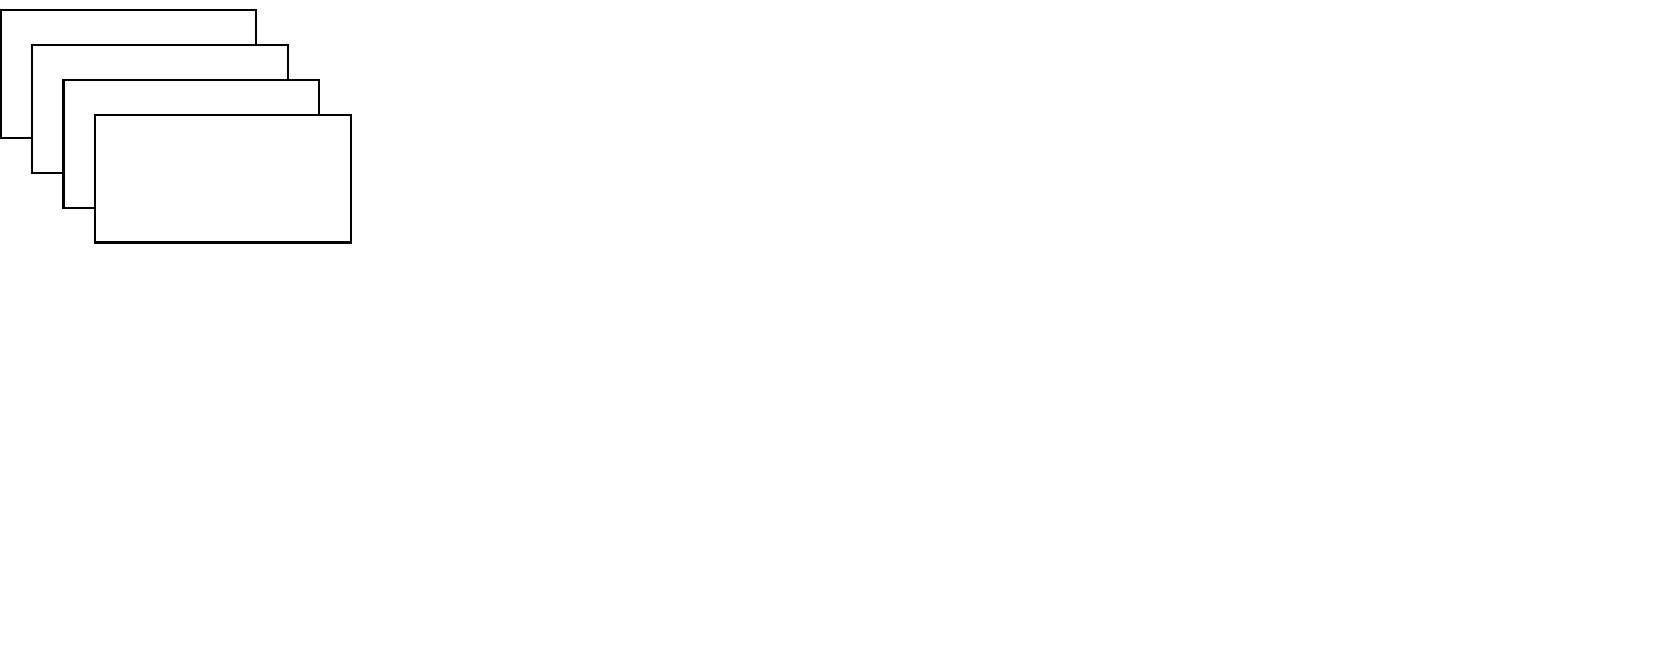
\includegraphics[width=0.8\linewidth]{img/pipeline_overview.pdf}
    \caption{The SfM pipeline: the pose estimation phase returns the cameras' 
    poses and the sparse points cloud. Then, the densification step uses 
    the input images and the previously camera's poses to create a dense
    point cloud.}
	\label{fig:pipeline_overview}
\end{figure}

\section{Pose Estimation}
\label{sec:pipeline_pose_estimation}
The cameras' poses estimation phase is similar to the classical visual 
odometry pipeline. The main differences lies in the variables' format and in 
the details concerning the procedures used.
For each new frame  (in the equirectangular format), we locate the
SURF keypoints \cite{bay2006surf}; we consider those keypoints whose inclination angle is in the range $[-60\degree; +60\degree]$. This is because the poles are affected by great 
distortions, thus robust matches outside this interval are rare.
Then, we look for matches in the last two frames and a filter performs some 
statistical analysis on the correspondences found and decides whether the frame 
is suitable for a robust pose estimation or not (in this case the frame is 
discarded).

If the frame is kept, its matches with the previous one are converted
and used for the essential matrix, $E$, estimation. Once $E$ is computed, 
it can be decomposed in the \([R|t]\) form where R is a rotation matrix 
and t is a translation vector up to an unknown scale factor.

The relative scale can be estimated thanks to the world points which have been 
triangulated thorough the matches and frame considered in previous pipeline 
iteration.

The pose for each camera can then be described as the composition of the 
motions between each view pair. We perform a bundle adjustment for the last 5 
poses in order to reduce the effect of drift.
Once every image has been processed by our pipeline, a final 
bundle adjustment is performed: it optimizes every camera pose estimated in order to 
further reduce drift error.

The coordinate system used in our pipeline is the one shown in 
Figure~\ref{fig:camera_model}, with the x-axis pointing right, the y-axis 
pointing down and the z-axis pointing forward.
We consider the spherical image divided in two hemispheres: front and back.
We call the image points 
whose 3rd component is positive, frontal points while we use the term rear 
points otherwise.
When we need to express spherical coordinates we use the same angles shown in 
Figure~\ref{fig:camera_model}:
the angle between the z-axis and the projection of $m$ on the xz-plane in 
the clock-wise direction is the longitude angle ($\lambda$) while the one 
between the negative y-axes and the same projection of $m$ is the latitude 
angle ($\phi$).

\begin{figure}
	\centering
	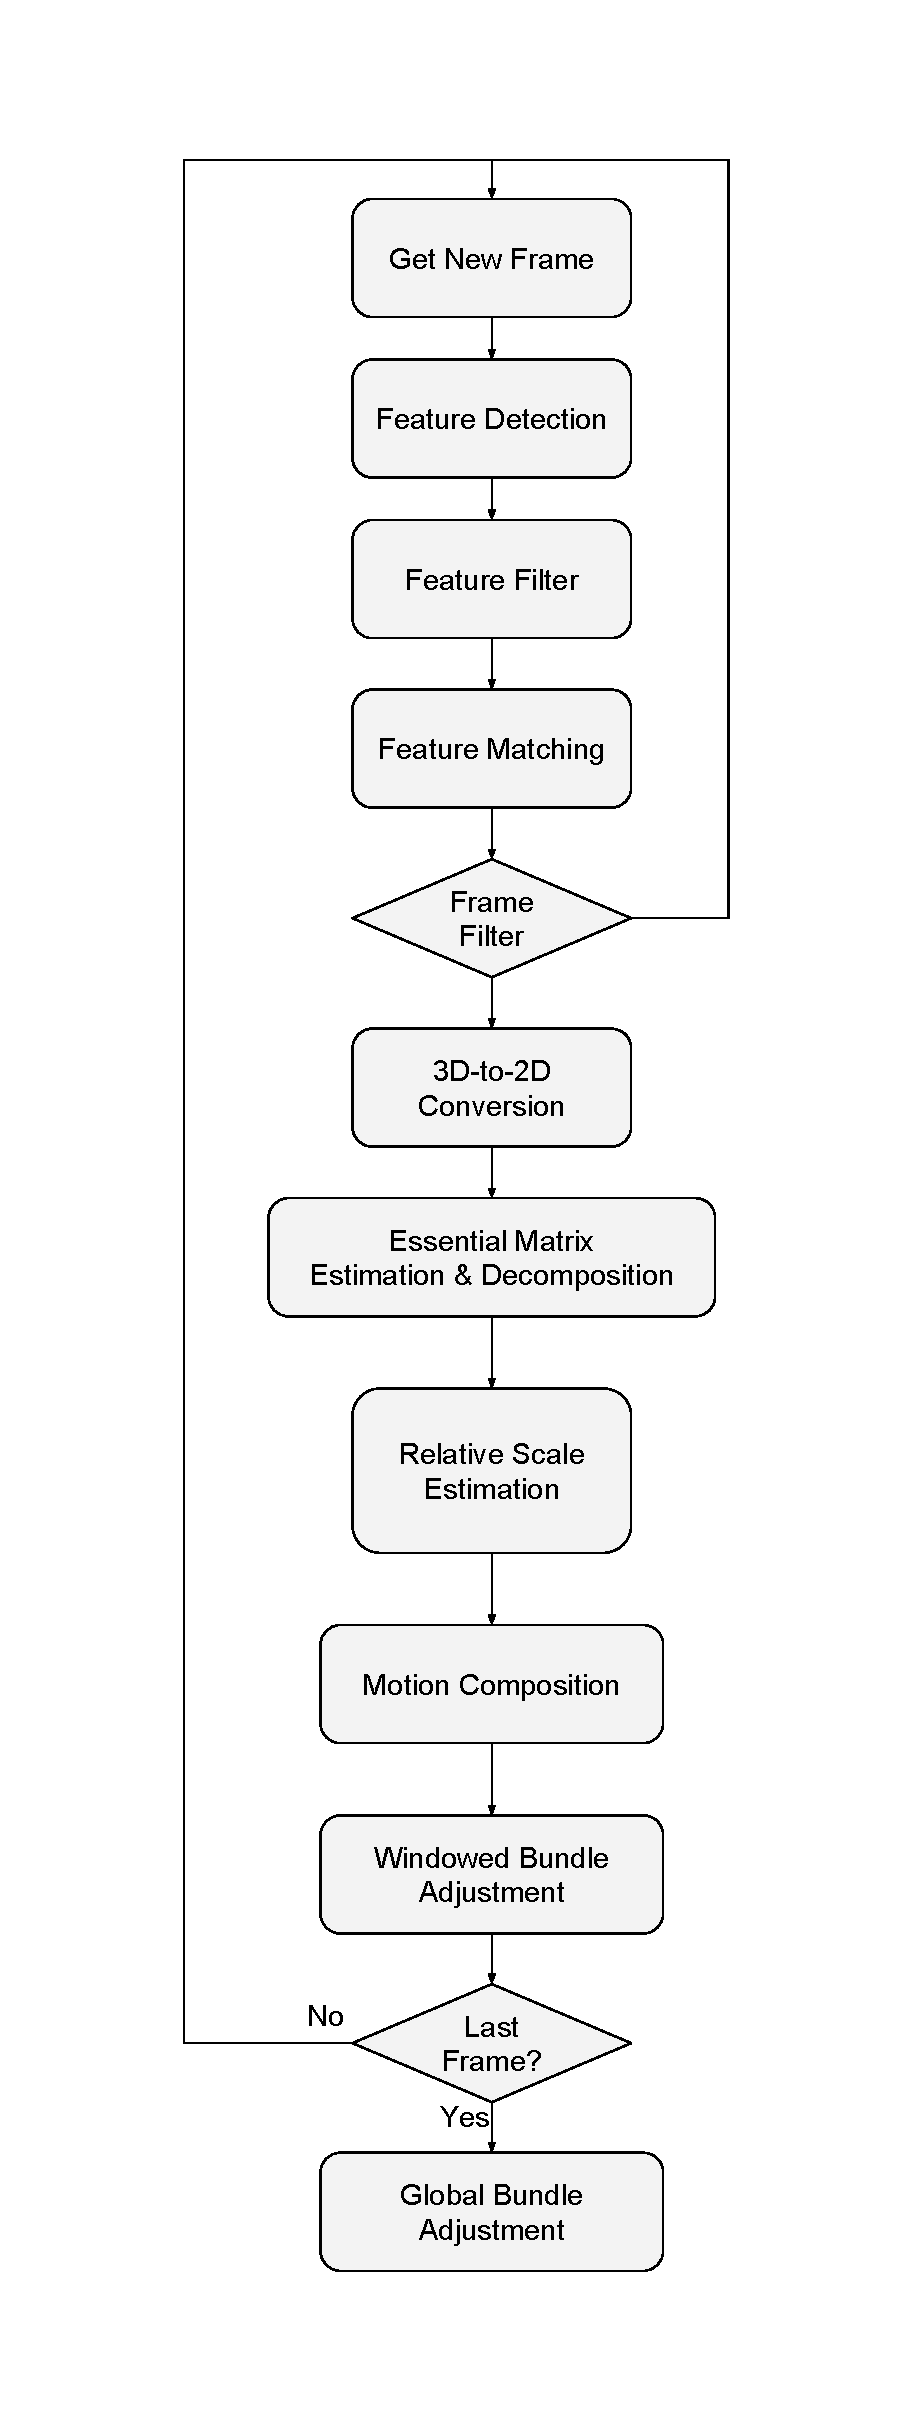
\includegraphics[width=0.5\linewidth]{img/sfm_block.pdf}
	\caption{A representation of the steps performed in the pose estimation 
	phase of our SfM pipeline.}
	\label{fig:sfm_block}
\end{figure}

\subsection{Key Points and Features Extraction}
In Section~\ref{sec:pipeline_pose_estimation} we introduced the need for 
features detection in order to find correspondences among the image pairs.
In our pipeline we use SURF features and descriptors 
\cite{bay2006surf}. SURF is a blob detector partly inspired by SIFT
\cite{lowe1999object};
It performs convolution on integral images with box filters in order to 
compute the Hessian matrix in scale space.
The descriptors exploits key point's neighborhood response to the Haar wavelet.
SURF, like SIFT, is patented but it can be used freely in non commercial
applications and for academic researches.
An implementation of the SURF detector is available in the MATLAB's Computer 
Vision Toolbox, and we employ it in our pipeline.

\subsection{Key Points Filtering}
The equirectangular format for spherical images introduces significant 
distortions in the areas around the poles. Interesting points in those areas 
are unlikely to match reliably with other points in a consecutive view, 
so they are just discarded.
Besides, in our experiments setup, the north and south poles usually point 
upward and downward respectively while most of the matches useful for pose 
estimation comes from the sides of the camera, so the removal of interesting 
points near the poles does not really affect the final result.

\subsection{Features Matching}
The matching strategy we carried out for equirectangular images is the same one 
adopted with standard images: two key points matches if the distance between 
their descriptors is less than a given threshold. Ambiguous matches 
are discarded if the ratio between the distances to the two closest matches is 
above a maximum.
We enforce matching robustness by forcing unique correspondences, that is:
only one feature in the first image can match with another one in the second
image. This is achieved with two passes of the matching procedure. During the 
first pass, each feature in the first images is checked for correspondences in
the second image; in the second pass, each features of the second image that 
has at least one correspondence in the first image is checked to see what 
interesting point of the first image it correspond to and the match with the
highest confidence is kept.

\subsection{Matches Filter}
In this step of the pipeline the matches are analyzed in order to decide 
whether a frame has to be kept because it is useful for motion estimation or
not.
We assume the environment considered for our studies is static: no people, 
cars or any kind of moving object is present in our scenes. In this case the 
apparent movement of corresponding objects in different views is caused by 
the camera motion only.
The filter computes the disparity between every correspondence found in the 
two views. It compares the median of the 20\% of the matches with the highest 
disparity value with a threshold. If such a median is above 
the threshold, the frame is kept for further processing in the pipeline, 
otherwise it is discarded.
The reason why we consider the correspondences with the greatest disparity is 
because, when the camera rotation is limited, the points that moves very little 
in consecutive views are usually far. The selection of these points for motion 
estimation can be counter-productive since they can easily produce numeric 
numerical errors. 

\subsection{3D-to-2D Key Points Conversion}
\label{sec:keypoints_conversion}
This step converts the key point format of equirectangular images to a new one 
suitable for the essential matrix estimation routine.
First the latitude and longitude coordinates of each feature point are 
extracted from the 2D mapping according to  
Equation~\ref{eq:ll2Cartesian_first}.
This equation returns the spherical coordinates for each feature point. 
We can then convert each of them to its cartesian format with 
Equation~\ref{eq:ll2Cartesian_second}. In order to estimate the essential 
matrix for each view pair, we use Equation~\ref{eq:epipolar_equation}, 
introduced by Longuet-Higgins in \cite{longuet1981computer}.
The point coordinates we obtain from Equation~\ref{eq:ll2Cartesian_first} and
Equation~\ref{eq:ll2Cartesian_second} do not need any normalization since there
is no intrinsic parameter for the full spherical camera model.

In order to exploit the routines to estimate the essential matrix available 
in the MATLAB's Computer Vision Toolbox, we need to perform an additional simple 
step.
Indeed this toolbox's routines deals with 2D images, thus they expect 
2D vectors when the input arguments are image points, however our camera
provides 3D image points.
We noticed that we can multiply the points $\myvec{p}$
and $\myvec{p}'$ by two 
scalars ${\lambda}$ and 
${\lambda}'$ and the equation is still valid. Thus, we obtain

\begin{equation*}
\lambda'\mathbf{p}'^\top E\lambda\mathbf{p} = 0 \text{.}
\end{equation*}

Therefore, we divide the 3D points obtained from the spherical images by their 
3rd component, discard it, and use the resulted 2D points as input for the 
MATLAB's essential matrix estimation routine, {\tt estimateEssentialMatrix}.

\begin{figure}
    \centering
    \def\svgwidth{0.8\columnwidth}
    \input{img/featurepoints_conversion.pdf_tex}
    \caption{A top view representation of the full spherical image's 
    different portions.
    The feature points that lie on the blue and green parts of the sphere are kept and,
    after the conversion described in Section~\ref{sec:keypoints_conversion},
    they are used for $E$ estimation. On the other hand, the points that lie
    on the red portions of the sphere are just discarded.
    Both the frontal point $p$ and the rear point $q$ are projected in $m$.}
	\label{fig:sphere_division}
\end{figure}

\subsubsection{Division by 3rd component vs. Projection}
It is worth to point out the differences between our method (division by the 3rd 
component of the vectors) and the perspective projection on a plane for feature
points conversion. Kangni et al. \cite{kangni2007orientation} converted the 
feature points extracted from spherical images to their projected images on a 
planar surface and used traditional techniques to estimate the camera poses.
Even though our method is very similar to \cite{kangni2007orientation}, there 
are some differences.
Projecting a point means that we have to deal with perspective geometry and its
parameters, like pixel size (or density), the principal point coordinates, 
focus length, image size, etc.
We can think of our method like a simplified perspective projection where
$f_x$ and $f_y$ are both set to 1, while $u_0$ and $v_0$ are 0.
The main difference between our method and a standard projection is that, if we
just divide each feature point by its 3rd component, we do not need to 
differentiate between frontal and rear points.
Figure~\ref{fig:sphere_division} shows how both the frontal point, $p$, and the 
rear one, $q$, are projected to the same point $m$ on the image plane.
This is not a problem, on the contrary, this helps the essential matrix 
estimation since it adds more redundant data to the input. We would obtain the
same estimation for $E$ if we used frontal (rear) points only.

The only thing we have to take care of is numerical error: if we divide by a 
small number, the result is affected by a large error. Therefore we
set a minimal value for the 3rd component magnitude a feature point must 
have in order for it to be used in motion estimation. 
We called this threshold parameter $z_{min}$.
The red part of the sphere in Figure~\ref{fig:sphere_division} are the ones
whose points are not considered for motion estimation, because their 
3rd component magnitude is below $z_{min}$.
Selecting points whose last component is above a certain threshold is 
equivalent to discarding those points that do not fit in the image plane
when projecting them.

The detailed theory about perspective projection is out of the scope of this 
thesis. It be found in \cite{szeliski2010computer} and \cite{Hartley2004}.

\subsection{Essential matrix estimation and decomposition}
As we described in the previous section, the essential matrix is estimated 
by the function {\tt estimateEssentialMatrix} of the MATLAB's 
Computer Vision Toolbox.
We use both frontal and rear image points for this estimation because
the increased number of correspondences between image pairs produces 
a more accurate result.

Once $E$ has been estimated, we need to decompose it in the 
\( [R|\myvec{t} ] \) form. This is again performed by a Computer Vision 
Toolbox's function: {\tt relativeCameraPose}.
The input for this function are the essential matrix computed before, the 
camera parameters and the matches found in the last two images.
The reason why this function needs the matches is because there are 4 possible 
SVD decomposition for the essential matrix. Each of this represents a 
different physical configuration for the cameras and world points.
In order to decide which decomposition is correct, the {\tt relativeCameraPose}
reprojects the matches in their corresponding world points according to each 
decomposition and selects the one that reprojects most of the correspondences in 
front of both cameras.
Since our cameras are full spherical and the image points belong to the 
rear hemisphere too, we need to provide as input to this function only 
those points that belongs to the frontal hemisphere. In this way, the routine 
can correctly estimate the camera's positions relatively to the set of frontal
points just like it would do for perspective cameras.
The reduced number of matching points for the input of the 
{\tt relativeCameraPose} function does not compromise the accuracy of the pose 
estimated, since those matches are used only to choose the 
correct SVD.

\subsection{Relative Scale Estimation}
Every relative motion between two views can only be estimated up to an unknown 
scale factor. Indeed the scale affects just the translation but still it has to 
be computed in order to create a coherent set of camera poses.
We obtain the relative scale with the formula from 
Equation~\ref{eq:relative_scale} \cite{scaramuzzaVisualOdometryI}.
That equation provides as many results as 3D points present in the last 3 
frames, thus, in order to compensate for the effects of outliers, we take the 
median.

\subsection{Motion Composition}
Once we have estimated the relative motion between two views, we use 
Equation~\ref{eq:motion_composition} to compute the new camera pose $C_n$ from 
the last estimated pose $C_{n-1}$ and the results $R_{n}$ and $t_n$ obtained 
from the decomposition of $E$.
We set the first orientation, $R_0$, to $I$ and the magnitude of the first 
translation, $t_0$, to 1.

\subsection{Windowed Bundle Adjustment}
Since every local motion is inevitably affected by error, the overall 
camera's path estimation tends to deviate from the real trajectory.
In order to reduce the drift and to get closer to a better starting point 
for the final bundle adjustment, every time we process a new frame, 
we perform a bundle adjustment over the last 5 poses.
This local optimization step on the most recent subset of frames is called
\textit{Windowed Bundle Adjustment}.

The bundle adjustment tries to reduce the sum of reprojection errors by changing the
world points, and camera positions. 
We keep the camera poses associated with the two oldest frames of the window 
fixed in order to prevent the adjustment from modifying the reconstruction's 
scale. This constraint also help by reducing the number of variables for the 
adjustment.

\subsection{Global Bundle Adjustment}
When all the views has been processed, we perform a final bundle adjustment 
step, in order to further reduce drift. Again, the first two poses are fixed in 
order to keep the relative scale.

\section{Point Cloud Densification}
\label{sec:pipeline_densification}
\todo[inline]{ancora da scrivere}
